\section{Présentation générale du projet}
\label{sec:pres-gener-du}

\subsection{Introduction}
\label{sec:introduction}

Dans le cadre de ce projet, il nous a été demandé d'implémenter un jeu de Pong sur
un Raspberry Pi 3.0 à l'aide d'un Sense HAT. \\

Vu la taille de la matrice du Sense HAT \textit{(de 8 LED's par 8)}, notre jeu de Pong subira
diverses modifications par rapport à la version officielle.

D'après les règles standards et les contraintes imposées, notre jeu de
Pong comportera les éléments suivants :

\begin{itemize}
\item un joystick pour guider la raquette;
\item un code couleur se rapportant au logo de la HEH (\textit{rouge et blanc});
\item l'affichage des points et des niveaux;
\item les rebonds de 45$^{\circ}$.
\end{itemize}

\subsection{Jeu de Pong}
\label{sec:jeu-de-pong}

D'un point de vue historique, le jeu de Pong est le premier jeu vidéo d'arcade
de sport créé. Celui-ci a été commercialisé en novembre 1972.

\begin{figure}[h]
  \centering
  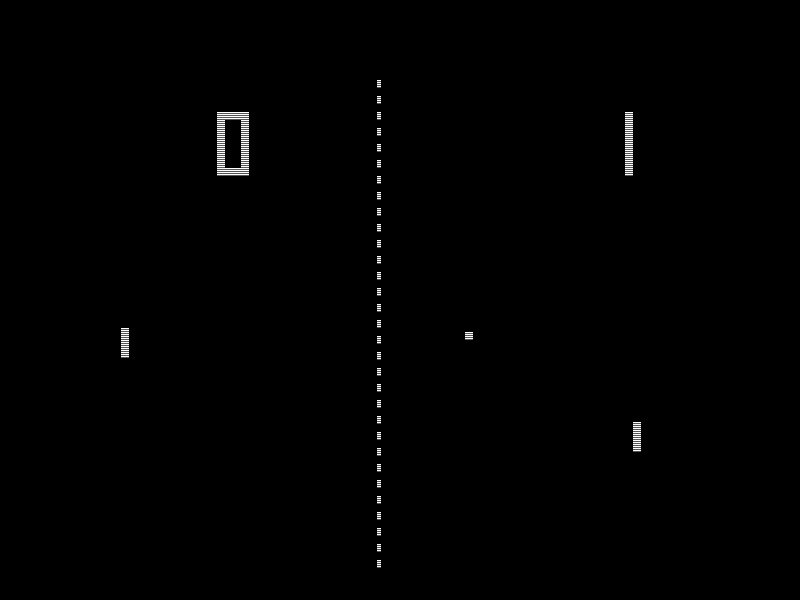
\includegraphics[scale=0.3]
  {textures/images/presentation/pong.png}
  \caption{Premier jeu de Pong}
  \label{fig:pong}
\end{figure}

Ce jeu est constitué de deux raquettes et d'une balle. Celle-ci ne peut toucher
que les murs supérieurs et inférieurs en effectuant un rebond selon un angle
déterminé. Lorsque la balle atteint le mur de gauche ou de droite, la partie est
terminée.

\newpage

\subsection{Modes de jeu}
\label{sec:modes-de-jeu}

Notre version du jeu de Pong propose deux modes :

\begin{itemize}
\item Un premier, disponible lors des deux premiers niveau où le joueur joue
contre un mur.

\begin{figure}[h]
  \centering
  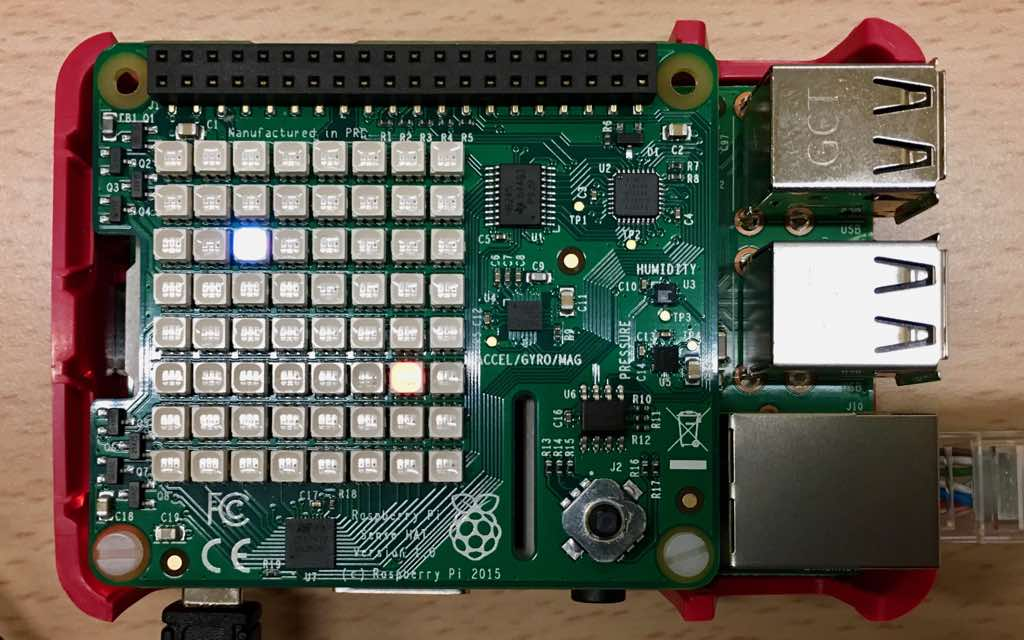
\includegraphics[scale=0.25]
  {textures/images/presentation/game1.jpg}
  \caption{Joueur contre mur}
  \label{fig:joueur-mur}
\end{figure}

\item Un deuxième, à partir du troisième niveau, permettant à une intelligence
artificielle (IA) de faire son apparition dans le jeu, augmentant les
similitudes avec le jeu de pong traditionnel.
\end{itemize}

\begin{figure}[h]
  \centering
  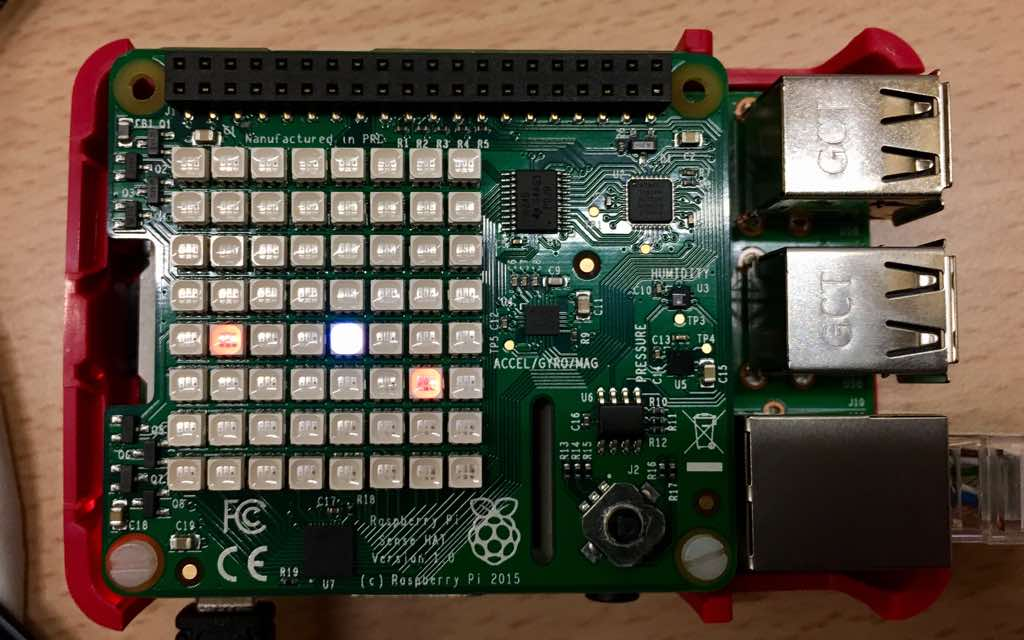
\includegraphics[scale=0.25]
  {textures/images/presentation/game2.jpg}
  \caption{Joueur contre IA}
  \label{fig:joueur-ia}
\end{figure}

\vspace{1cm}

\underline{Remarque :} la vitesse du jeu augmente progressivement à chaque jeu. \\
De même, elle augmente lors du passage au niveau supérieur.

\newpage

\subsection{Raspberry Pi}
\label{sec:raspbeery-pi}

Le Raspberry Pi \footnote{\url{https://www.raspberrypi.org/}} est un
nano-ordinateur équipé d'un microprocesseur ARM.

\begin{figure}[h]
  \centering
  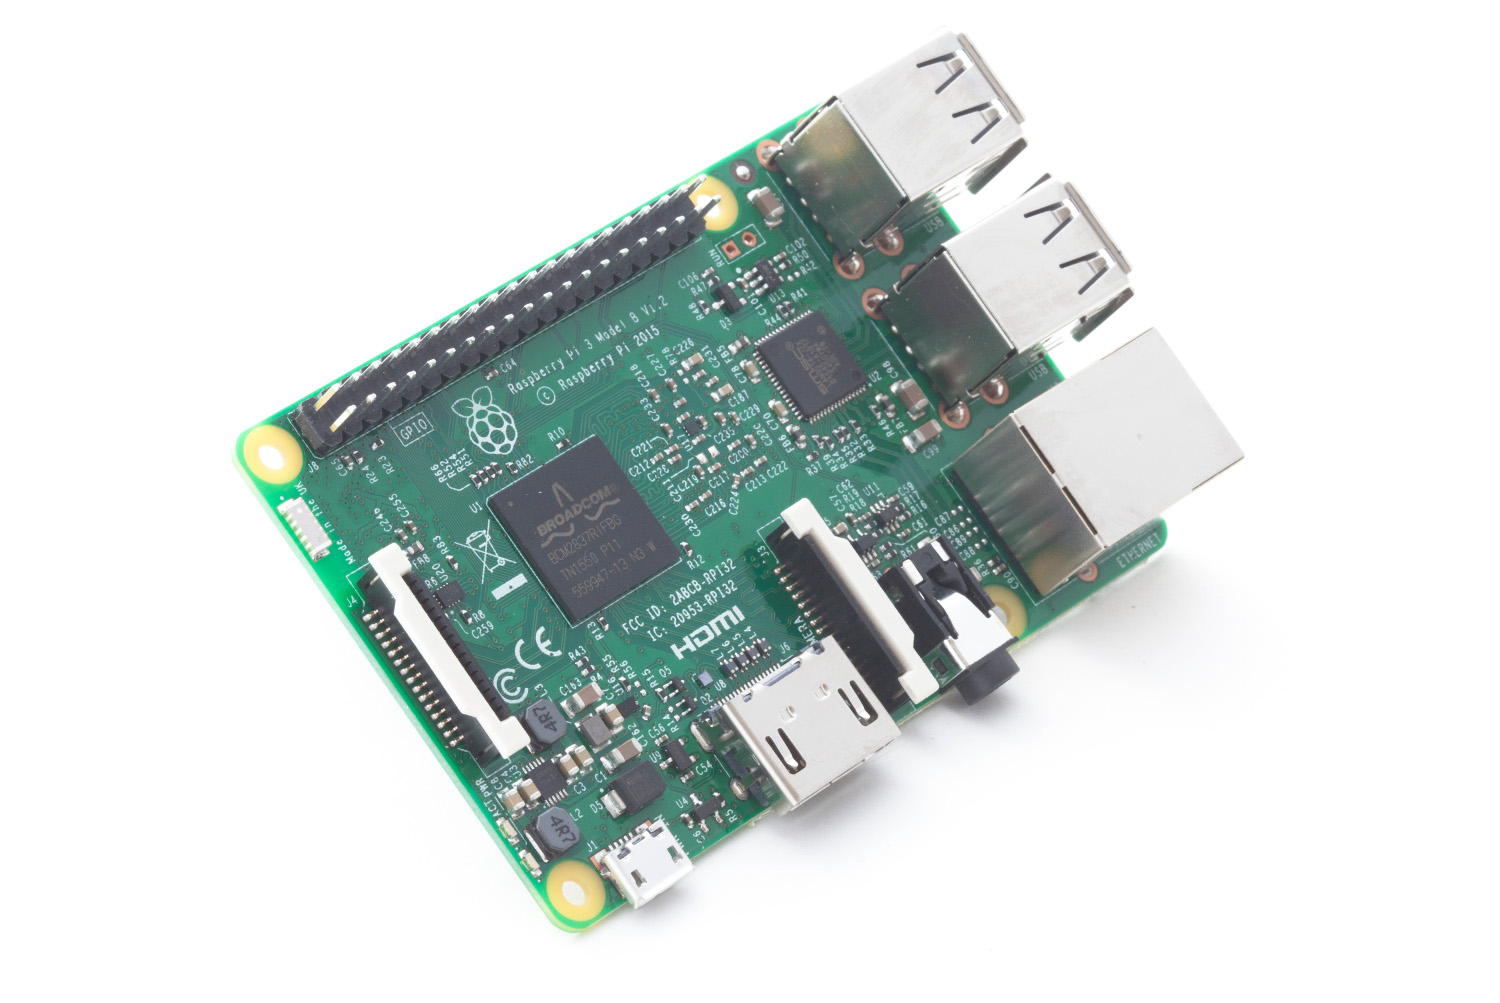
\includegraphics[scale=0.18]
  {textures/images/presentation/raspberry.jpg}
  \caption{Raspberry Pi, Modèle 3 B}
  \label{fig:raspberry-pi}
\end{figure}

En raison de sa très faible consommation en énergie, celui-ci est majoritairement
utilisé en tant que serveur, puisqu'il peut tourner jour et nuit pour un coût de
quelques euros par an en électricité.

Concernant l'installation du système d'exploitation, il est fortement conseillé
d'utiliser un noyaux Linux avec une distribution compatible telles que Raspbian,
Debian, Ubuntu MATE, etc.

Après l'installation, nous avons connecté le Raspberry Pi au routeur afin de
connaître son adresse IP par défaut afin de pouvoir modifier celle-ci à l'aide
du fichier \\ \textit{/boot/cmdline.txt}. De même, nous avons modifié son nom
dans le but de simplifier l'identification de celui-ci lors de son utilisation ultérieure.

\newpage

\subsection{Sense HAT}
\label{sec:sense-hat}

\begin{figure}[h]
  \centering
  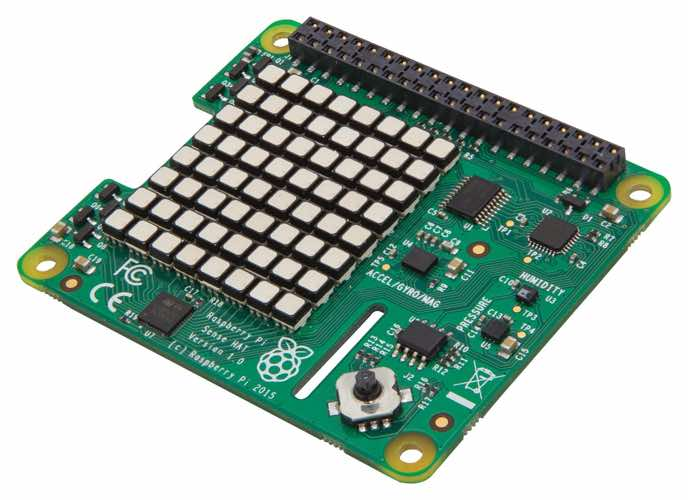
\includegraphics[scale=0.35]
  {textures/images/presentation/senseHAT.jpg}
  \caption{Sense HAT}
  \label{fig:sense-hat}
\end{figure}

Le Sense HAT \footnote{\url{https://www.raspberrypi.org/products/sense-hat/}}
est une carte additionnelle qui dispose d'une matrice LED 8x8, d'un joystick à cinq
boutons et comprend les capteurs suivants :

\begin{itemize}
\item Gyroscope
\item Accéléromètre
\item Magnétomètre
\item Température
\item Pression barométrique
\item Humidité
\end{itemize}

\underline{Remarque :} une librairie permettant
d'interagir avec les différents capteurs est disponible en Python.

Pour l'anecdote, le Sense HAT a été spécialement conçu pour la mission Astro Pi
\footnote{\url{https://astro-pi.org/}} lancé à la station spatiale
internationale en décembre 2015.

%%% Local Variables:
%%% mode: latex
%%% TeX-master: t
%%% End:
